%% This is a tikz file

% This file is set up to use 11pt palatino font.
\tikzset{node lower left/.style={font=\scriptsize,anchor=north east,yshift=-0.032cm,text height=0.198cm,text depth=0.079cm,inner sep=0.03cm},
leaf/.style={font=\normalsize,anchor=west,text height=0.271cm,text depth=0.109cm,inner sep=0.13cm},
node upper left/.style={font=\scriptsize,anchor=south east,yshift=-0.032cm,text height=0.198cm,text depth=0.079cm,inner sep=0.03cm},
bracket label/.style={font=\normalsize,anchor=west,text height=0.271cm,text depth=0.109cm,inner sep=0.2cm},
node upper right/.style={font=\scriptsize,anchor=south west,text height=0.198cm,text depth=0.079cm,inner sep=0.03cm},
node right/.style={font=\scriptsize,anchor=west,text height=0.198cm,text depth=0.079cm,inner sep=0.03cm},
branch/.style={font=\tiny,text height=0.149cm,text depth=0.059cm,inner sep=0.025cm},
root/.style={font=\normalsize,anchor=east,text height=0.271cm,text depth=0.109cm},
node lower right/.style={font=\scriptsize,anchor=north west,text height=0.198cm,text depth=0.079cm,inner sep=0.03cm}}
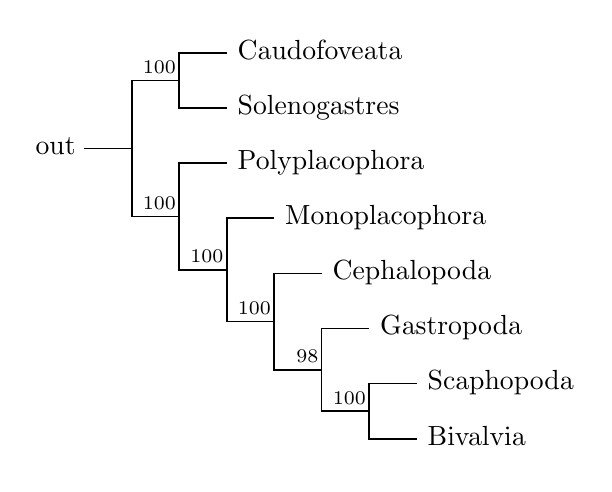
\begin{tikzpicture}[semithick,inner sep=0.1cm]
%                         +---------2:Caudofoveata
%               +---------1:100
%               |         +---------3:Solenogastres
% out:4---------0
%               |         +---------6:Polyplacophora
%               |         |
%               +---------5:100     +---------8:Monoplacophora
%                         |         |
%                         +---------7:100     +---------10:Cephalopoda
%                                   |         |
%                                   +---------9:100     +---------12:Gastropoda
%                                             +---------11:98
%                                                       |         +----------14:Scaphopoda
%                                                       +---------13:100
%                                                                 +----------15:Bivalvia

% The scale is 6.030000, and the yScale is 0.700000

%% Coordinates of nodes.
\coordinate (n4) at (0.000,3.686);
\coordinate (n0) at (0.603,3.686);
\coordinate (n0p) at (0.000,3.686);
\coordinate (n1) at (1.206,4.550);
\coordinate (n1p) at (0.603,4.550);
\coordinate (n2) at (1.809,4.900);
\coordinate (n2p) at (1.206,4.900);
\coordinate (n3) at (1.809,4.200);
\coordinate (n3p) at (1.206,4.200);
\coordinate (n5) at (1.206,2.822);
\coordinate (n5p) at (0.603,2.822);
\coordinate (n6) at (1.809,3.500);
\coordinate (n6p) at (1.206,3.500);
\coordinate (n7) at (1.809,2.144);
\coordinate (n7p) at (1.206,2.144);
\coordinate (n8) at (2.412,2.800);
\coordinate (n8p) at (1.809,2.800);
\coordinate (n9) at (2.412,1.487);
\coordinate (n9p) at (1.809,1.487);
\coordinate (n10) at (3.015,2.100);
\coordinate (n10p) at (2.412,2.100);
\coordinate (n11) at (3.015,0.875);
\coordinate (n11p) at (2.412,0.875);
\coordinate (n12) at (3.618,1.400);
\coordinate (n12p) at (3.015,1.400);
\coordinate (n13) at (3.618,0.350);
\coordinate (n13p) at (3.015,0.350);
\coordinate (n14) at (4.221,0.700);
\coordinate (n14p) at (3.618,0.700);
\coordinate (n15) at (4.221,0.000);
\coordinate (n15p) at (3.618,0.000);

%% horizontal lines
\draw (n0p) -- (n0);
\draw (n1p) -- (n1);
\draw (n2p) -- (n2);
\draw (n3p) -- (n3);
\draw (n5p) -- (n5);
\draw (n6p) -- (n6);
\draw (n7p) -- (n7);
\draw (n8p) -- (n8);
\draw (n9p) -- (n9);
\draw (n10p) -- (n10);
\draw (n11p) -- (n11);
\draw (n12p) -- (n12);
\draw (n13p) -- (n13);
\draw (n14p) -- (n14);
\draw (n15p) -- (n15);

%% vertical lines
\draw [line cap=rect] (n1p) -- (n5p);
\draw [line cap=rect] (n2p) -- (n3p);
\draw [line cap=rect] (n6p) -- (n7p);
\draw [line cap=rect] (n8p) -- (n9p);
\draw [line cap=rect] (n10p) -- (n11p);
\draw [line cap=rect] (n12p) -- (n13p);
\draw [line cap=rect] (n14p) -- (n15p);

%% leaf labels
\node [leaf,text height=0.271cm,text depth=0.109cm] at (n2) {Caudofoveata};
\node [leaf,text height=0.271cm,text depth=0.109cm] at (n3) {Solenogastres};
\node [leaf,text height=0.271cm,text depth=0.109cm] at (n6) {Polyplacophora};
\node [leaf,text height=0.271cm,text depth=0.109cm] at (n8) {Monoplacophora};
\node [leaf,text height=0.271cm,text depth=0.109cm] at (n10) {Cephalopoda};
\node [leaf,text height=0.271cm,text depth=0.109cm] at (n12) {Gastropoda};
\node [leaf,text height=0.271cm,text depth=0.109cm] at (n14) {Scaphopoda};
\node [leaf,text height=0.271cm,text depth=0.109cm] at (n15) {Bivalvia};

%% root label
\node [root,text height=0.271cm,text depth=0.109cm] at (n4) {out};

% internal node labels (doSmartLabels is True)
\node [node upper left,text height=0.198cm,text depth=0.079cm] at (n1) {100};
\node [node upper left,text height=0.198cm,text depth=0.079cm] at (n5) {100};
\node [node upper left,text height=0.198cm,text depth=0.079cm] at (n7) {100};
\node [node upper left,text height=0.198cm,text depth=0.079cm] at (n9) {100};
\node [node upper left,text height=0.198cm,text depth=0.079cm] at (n11) {98};
\node [node upper left,text height=0.198cm,text depth=0.079cm] at (n13) {100};

\end{tikzpicture}
